\chapter{Aluminum Nitride as a Platform to Support RV Spectroscopy} \label{chapter:astro-comb}

\section{Introduction} \label{astro-comb:intro}

The study of precise and accurate synthetic wavelength calibrators---sometimes endearingly called astro-combs when applied to RV spectrographs---have been critical to the steady improvement in RV measurement precision.

In this Chapter, I introduce aluminum nitride as another technology for possible inclusion in future astro-comb development and application. In Chapter \ref{astro-comb:aln}, I provide some background on aluminum nitride and why it is promising for use in visible radial-velocity spectroscopy. In Chapter \ref{astro-comb:micro-ring}, I describe testing completed with an aluminum nitride micro-ring on EXPRES to confirm comb viability in blue and ultraviolet wavelength regions. Finally, in Chapter \ref{astro-comb:eom}, I provide details on a high repetition-rate electro-optic modulation comb built to test aluminum nitride waveguides for potential application with visible-wavelength spectrographs.

\section{Aluminum Nitride} \label{astro-comb:aln}



Optical nonlinearity is a strong tool that can be used on this near-infrared EOM comb to expand it into the visible spectrum. Second-order nonlinearities provide second harmonic generation (SHG), a specific form of sum frequency generation (SFG), that doubles the frequency of light incident on the nonlinear material (Figure \ref{fig:sfg_example}(b)). Similarly, third-order nonlinearities provide third harmonic generation (THG) that triples the incident light frequency (Figure \ref{fig:sfg_example}(c)). Silicon dioxide and silicon nitride (SiN), historically the most widely researched nonlinear waveguide materials, only have strong third-order nonlinearity. Aluminum nitride (AlN), on the other hand, is quickly gaining ground as a phenomenal material for on-chip nonlinear optics applications because it has both strong third-order and second-order nonlinearity as well as low loss over an extremely wide bandwidth from the ultraviolet to the mid-infrared \citep{Jung2016}. Therefore, AlN is ideally suited for application to a broadband astro-comb.

\begin{figure}
    \centering
    \includegraphics[width=0.6\textwidth]{images/sfg_example.png}
    \caption{Diagram of nonlinear optical multi-harmonic generation demonstrated by an AlN on-chip microring resonator. (a) Cascaded four-wave mixing NIR comb produced by the whispering gallery modes (unrelated to the proposed astro-comb) centered at 1550 nm. (b) Second order nonlinear effects produce a comb centered at 725 nm. (c) Third order nonlinear effects produce a comb centered at 517 nm. Image reprinted from \cite{Jung2014a}}
    \label{fig:sfg_example}
\end{figure}

The Yale Nanodevices Laboratory (YNDL) has developed a mature nanofabrication process for AlN that deposits the material with a predetermined geometry onto silicon nitride chips. Using this device, the YNDL has fabricated many on-chip AlN waveguides with varying lengths \citep[\SI{300}{\micro\meter} to \SI{3}{\centi\meter};][]{Xiong2012a}, thicknesses \citep[330--\SI{1500}{\nano\meter};][]{Pernice2012}, and shapes (e.g. differing radii of curvature). These tests also showed strong SHG in the AlN waveguides with differing wavelength-dependent throughput based on the associated geometries. More recently, the YNDL has also explored AlN microring resonators \citep{Jung2013, Guo2016}. For example, \citet{Jung2014a} demonstrated an AlN microring resonator that generated a green, red, and infrared FC using the Yale Exoplanet Laboratory (YEL) in-lab high-resolution spectrograph. The span of this comb is detailed in Figure \ref{fig:sfg_example}. Although the microresonator FC is not stabilized as of yet, it proves that sufficient power could be produced by the SHG and THG frequencies in AlN for detection by a RV spectrograph (with future research looking to stretch this to fourth harmonic generation).



AlN is also an excellent candidate for supercontinuum (SC) generation, the phenomenon where an incident narrow-band laser pulse experiences extreme spectral broadening when propagated through a nonlinear optical material \citep{Dudley2006}. The Menlo LFC actually uses SC generation, through a photonic crystal fiber (PCF), to produce its visible-spanning FC \citep{Probst2014}. However, the EXPRES group has found that this comb does not stretch below \SI{480}{\nano\meter} very reliably, with stated issues of PCF burning for blue and ultraviolet light. The YNDL, on the other hand, has shown promising preliminary results where a SC generated with an AlN waveguide and an \SI{80}{\mega\hertz} pulse laser produces blue and ultraviolet lines below \SI{450}{\nano\meter}. 



Therefore, I am proposing to develop an affordable, compact, and direct-generation optical FC (or ``astro-comb'') that extends from the near-ultraviolet to the mid-infrared ($\sim$350–-\SI{2500}{\nano\meter}). This astro-comb will utilize two technologies that have been already been thoroughly developed:
\begin{enumerate}
    \item a near-infrared electro-optic modulation (EOM) FC, and
    \item an aluminum nitride (AlN) on-chip waveguide that uses nonlinear material properties to broaden the EOM FC.
\end{enumerate}
Upon completion, this technology will be able to calibrate a wide range of RV spectrographs to $10^{-11}$ precision (corresponding to \SI{1}{\centi\meter\per\second} RV on EXPRES for example) in the search for Earth-like exoplanets orbiting sun-like stars. Such a laser frequency comb has not yet been introduced to the RV community, therefore any contribution I can make towards its completion would be a significant part of my thesis. This section begins with brief descriptions of the current advancement of both the EOM comb and AlN waveguides (Section \ref{subsec:astro-comb_bkgd}), followed by my preliminary comb design and plans for testing (Section \ref{subsec:comb_design}).

\section{AlN Micro-ring}\label{astro-comb:micro-ring}

The most important aspect of AlN's potential usability with spectrograph systems such as EXPRES is its ability to convert infrared light efficiently and transparently throughout the entire band-pass of the instrument. As noted in Chapter \ref{intro:wvln_cal}, the Menlo LFC used with EXPRES has a stated band-pass of 450--750\nm, though in practice this has been shown to be closer to 500--720\nm. Therefore, demonstration of 

I have also tested a more updated version of this microring resonator with EXPRES both when it was being commissioned in the Yale Exoplanet Lab and at the Discovery Channel Telescope. An example of one of the spectra taken is shown in Figure \ref{fig:aln_spectrum}. SHG lines are suppressed by an \SI{700}{\nano\meter} edgepass filter. However, there are clearly THG lines near \SI{500}{\nano\meter} and even a significant number of lines below the \SI{450}{\nano\meter} boundary that many other nonlinear optical materials (such as silicon dioxide and nitride) cannot seem to cross. These results are extremely promising for AlN's use as a SFG waveguide.

\begin{figure}
    \centering
    \includegraphics[width=\textwidth]{figures-3/aln_spectrum.png}
    \caption{Spectrum of an AlN microring measured with EXPRES.}
    \label{fig:aln_spectrum}
\end{figure}

\section{Electro-optic Modulation Comb} \label{astro-comb:eom}

\begin{figure}
    \centering
    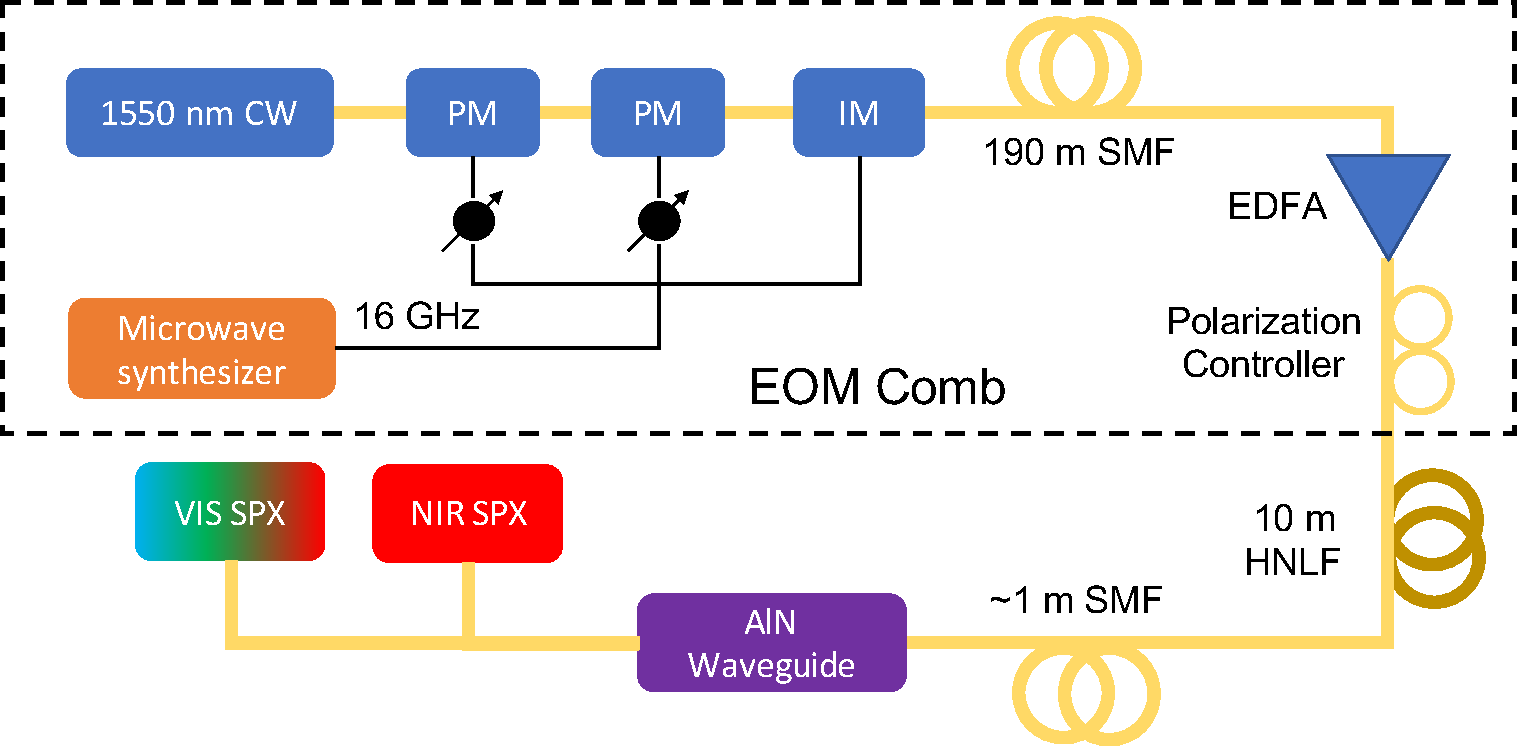
\includegraphics[width=\textwidth]{figures-3/eom-diagram.pdf}
    \caption[Electro-optic modulation comb schematic diagram]{Schematic diagram of the EOM built for testing with AlN waveguides.}
    \label{fig:eom-diagram}
\end{figure}



\section{Summary and Discussion}




Special thanks to Alex Bruch for his significant guidance in learning the ins and outs of non-linear optics as well as the contribution of his simulation code to this chapter and for joining me in collecting micro-comb data with EXPRES. I would also like to thank Zheng Gong for his help in working with the EOM comb. I would finally like to thank Scott Diddams and Stephanie Leifer for their guidance through the EOM prototyping process.